\documentclass[12pt]{article}
\usepackage[utf8]{inputenc}
\usepackage{graphicx}
\usepackage{subcaption}
\usepackage{amsmath}
\usepackage{fancyhdr}
\usepackage{geometry}
\usepackage{float}
\usepackage{listings}
\usepackage{xcolor}
\usepackage{array}
\usepackage{caption}
\usepackage{booktabs}
\usepackage[english]{babel}
\usepackage{amssymb}
\usepackage{hyperref}

\lstset{
    basicstyle=\ttfamily\footnotesize,
    backgroundcolor=\color{gray!10},
    keywordstyle=\color{blue},
    commentstyle=\color{green!50!black},
    stringstyle=\color{red},
    numbers=left,
    numberstyle=\tiny\color{gray},
    stepnumber=1,
    numbersep=10pt,
    showstringspaces=false,
    frame=single,
    tabsize=4,
    breaklines=true,
    breakatwhitespace=false,
    language=Python
}

\linespread{1.25}
\setlength{\parindent}{0.8cm}
\setlength{\parskip}{0em}
\renewcommand{\headrulewidth}{0pt}
\geometry{a4paper, portrait, margin=1in}
\setlength{\headheight}{14.49998pt}
\graphicspath{{Lab3/charts/}}

\begin{document}

% ─── TITLE PAGE ───────────────────────────────────────────────────────────────
\begin{titlepage}
  \begin{center}
    \textbf{\large Ministry of Education of Republic of Moldova}\\[0.1cm]
    \textbf{\large Technical University of Moldova}\\[0.1cm]
    \textbf{\large Faculty of Computers, Informatics and Microelectronics}\\[1.2cm]

    \vspace{40mm}

    \textsc{\Large Laboratory Work 3:}\\[0.2cm]
    \textsc{\Large Empirical Analysis of Graph Traversal Algorithms}\\[0.2cm]
    \textsc{\large Depth-First Search (DFS) and Breadth-First Search (BFS)}\\[0.4cm]

    \vspace{65mm}

    \begin{minipage}[t]{0.4\textwidth}
      \begin{flushleft}\large
        \emph{Author:}\\
        st. gr. FAF-242\\[0.4cm]
        \emph{Verified:}\\
        asist. univ.
      \end{flushleft}
    \end{minipage}
    ~
    \begin{minipage}[t]{0.4\textwidth}
      \begin{flushright}\large
        \emph{}\\
        Tacu Igor\\[0.4cm]
        \emph{}\\
        Fiștic Cristofor
      \end{flushright}
    \end{minipage}\\[2cm]

    \vspace{5mm}
    \large Chișinău -- 2026

    \vfill
  \end{center}
\end{titlepage}

% ─── TABLE OF CONTENTS ────────────────────────────────────────────────────────
\clearpage
\thispagestyle{empty}
\tableofcontents

\clearpage
\setcounter{page}{2}
\pagestyle{fancy}
\fancyhf{}
\rhead{\thepage}

% ─── 1. OBJECTIVE ─────────────────────────────────────────────────────────────
\section*{OBJECTIVE}
\addcontentsline{toc}{section}{OBJECTIVE}

Study and empirically analyse the two fundamental graph traversal algorithms ---
Breadth-First Search (BFS) and Depth-First Search (DFS) --- measuring their execution
time and memory consumption across multiple graph structures and sizes, and identify
each algorithm's strengths and limitations in practice.

\subsection*{Tasks}
\addcontentsline{toc}{subsection}{Tasks}

\begin{enumerate}
  \item Implement BFS, DFS (iterative), and DFS (recursive) in Python.
  \item Define the graph properties (types and sizes) against which the analysis is performed.
  \item Select metrics for comparison: execution time and peak auxiliary-structure size.
  \item Run each algorithm on five graph types across a range of node counts.
  \item Generate graphical presentations of the collected data.
  \item Produce animated GIF demonstrations of BFS and DFS traversal on a demo graph.
  \item Test both algorithms on edge-case inputs (empty graph, single node, disconnected
        graph, self-loops, complete graph).
  \item Deduce conclusions from the obtained data.
\end{enumerate}

% ─── 2. THEORETICAL BACKGROUND ───────────────────────────────────────────────
\section*{THEORETICAL BACKGROUND}
\addcontentsline{toc}{section}{THEORETICAL BACKGROUND}

\subsection*{Empirical Analysis}
\addcontentsline{toc}{subsection}{Empirical Analysis}

\hspace{0.8cm} Empirical analysis is an experimental approach to measuring algorithm
efficiency. Instead of deriving bounds through mathematical reasoning alone, the
algorithm is implemented, executed on controlled input datasets, and the observed
metrics are recorded and plotted. This is especially useful when:

\begin{itemize}
  \item the theoretical analysis is complex or input-dependent;
  \item comparing practical performance of algorithms with identical asymptotic complexity;
  \item assessing the impact of data structure constants and implementation choices.
\end{itemize}

Each algorithm was run \textbf{7 times} per (graph type, size) pair and the
\textbf{mean} time in milliseconds was recorded to smooth out OS-scheduling noise.

\subsection*{Algorithm Overviews}
\addcontentsline{toc}{subsection}{Algorithm Overviews}

\hspace{0.8cm} Both BFS and DFS are linear-time graph traversal algorithms with the
same asymptotic complexity but fundamentally different traversal orders and memory
access patterns.

\textbf{Breadth-First Search (BFS)} explores the graph level by level.  Starting
from the source node it visits all neighbours at distance 1, then all at distance 2,
and so on.  It uses a \textit{queue} (FIFO) as the auxiliary structure.  Because it
always processes the closest unvisited node first, BFS guarantees finding the
\emph{shortest path} (in terms of hop count) from the source to any reachable node in
an unweighted graph.  Its peak queue size is proportional to the \emph{width} (maximum
level size) of the traversal tree.

\textbf{Depth-First Search (DFS)} explores the graph by going as deep as possible
along each branch before backtracking.  It uses a \textit{stack} (LIFO) --- either an
explicit stack (iterative version) or the call stack (recursive version).  DFS is
well-suited for cycle detection, topological sorting, and connectivity analysis.  Its
peak stack depth is proportional to the \emph{depth} of the traversal tree.

\begin{center}
\renewcommand{\arraystretch}{1.4}
\begin{tabular}{lcccc}
\toprule
\textbf{Algorithm} & \textbf{Time} & \textbf{Space (aux)} & \textbf{Ordering} & \textbf{Shortest path?} \\
\midrule
BFS           & $O(V + E)$ & $O(V)$ --- queue width  & Level-order  & Yes \\
DFS (iter.)   & $O(V + E)$ & $O(E)$ --- stack (w/ dup.) & Depth-first & No  \\
DFS (rec.)    & $O(V + E)$ & $O(V)$ --- call stack depth & Depth-first & No  \\
\bottomrule
\end{tabular}
\captionof{table}{Theoretical time and space complexity of BFS and DFS.}
\end{center}

\noindent\textit{Note:} The iterative DFS implemented here pushes neighbours onto the
stack before checking whether they have been visited (the visited check happens on pop).
This means the explicit stack can contain duplicate entries and grow to $O(E)$ on dense
graphs, unlike recursive DFS whose call stack is bounded by $O(V)$ (the maximum
recursion depth).

% ─── 3. INPUT FORMAT ──────────────────────────────────────────────────────────
\section*{INPUT FORMAT}
\addcontentsline{toc}{section}{INPUT FORMAT}

\hspace{0.8cm} Five graph types were chosen to capture a broad range of structural
properties:

\begin{enumerate}
  \item \textbf{Sparse random} -- undirected graph, average degree $\approx 2$
        (edge probability $p = 2/(n-1)$). Represents real-world sparse networks.
        Sizes: $n \in \{10,\,50,\,100,\,250,\,500,\,1000,\,2000,\,5000\}$.

  \item \textbf{Dense random} -- undirected graph, edge probability $p = 0.30$.
        Represents highly connected networks; $O(n^2)$ edge count.
        Sizes: $n \in \{10,\,50,\,100,\,250,\,500,\,1000\}$.

  \item \textbf{Complete binary tree} -- balanced tree with $n$ nodes (node $i$
        has children $2i+1$ and $2i+2$).  Represents hierarchical data; depth
        $= \lfloor \log_2 n \rfloor$.
        Sizes: same as sparse.

  \item \textbf{Grid graph} -- $\sqrt{n} \times \sqrt{n}$ square grid, each
        interior node connected to its four neighbours.  Represents spatial
        graphs; BFS explores expanding rings.
        Sizes (actual $n$): $\{9,\,25,\,64,\,100,\,225,\,400,\,625,\,900,\,1600,\,2500\}$.

  \item \textbf{Chain graph} -- linear path $0 \!-\! 1 \!-\! 2 \!-\! \cdots \!-\! (n\!-\!1)$.
        Worst-case depth for recursive DFS; both BFS and iterative DFS process one
        node per step.
        Sizes: same as sparse.
\end{enumerate}

All graphs were generated with a fixed random seed (42) for reproducibility.
Disconnected graphs were made connected by linking any isolated node to a
uniformly-random node in the already-reachable component.

% ─── 4. IMPLEMENTATION ────────────────────────────────────────────────────────
\section*{IMPLEMENTATION}
\addcontentsline{toc}{section}{IMPLEMENTATION}

\hspace{0.8cm} All three algorithms were implemented in Python using a standard
adjacency-list representation (\texttt{dict[int, list[int]]}).  Each function
returns a result dictionary containing the visit order, elapsed time in
milliseconds, peak auxiliary-structure size, and total nodes visited.

\subsection*{BFS}
\addcontentsline{toc}{subsection}{BFS}

\hspace{0.8cm} BFS uses \texttt{collections.deque} for O(1) \texttt{popleft()}
operations.  Nodes are marked visited \emph{when enqueued} (not when dequeued),
preventing duplicate queue entries and ensuring O(V) peak queue size.

\begin{lstlisting}[caption={Breadth-First Search}, label={lst:bfs}]
def bfs(graph: dict, start) -> dict:
    visited   = {start}
    queue     = deque([start])
    order     = []
    max_queue = 1

    t0 = time.perf_counter()
    while queue:
        node = queue.popleft()
        order.append(node)
        for nbr in graph.get(node, []):
            if nbr not in visited:
                visited.add(nbr)
                queue.append(nbr)
                if len(queue) > max_queue:
                    max_queue = len(queue)
    elapsed_ms = (time.perf_counter() - t0) * 1_000

    return {"order": order, "time_ms": elapsed_ms,
            "max_queue": max_queue, "nodes_visited": len(order)}
\end{lstlisting}

\subsection*{DFS -- Iterative}
\addcontentsline{toc}{subsection}{DFS -- Iterative}

\hspace{0.8cm} The iterative DFS uses a Python list as an explicit stack.  Neighbours
are pushed in reverse-sorted order so that the traversal order matches the recursive
version.  The visited check is performed \emph{on pop} (not on push), which is the
standard iterative pattern but can cause the stack to hold duplicate entries on dense
graphs.

\begin{lstlisting}[caption={DFS -- Iterative (explicit stack)}, label={lst:dfs-iter}]
def dfs_iterative(graph: dict, start) -> dict:
    visited   = set()
    stack     = [start]
    order     = []
    max_stack = 1

    t0 = time.perf_counter()
    while stack:
        node = stack.pop()
        if node in visited:
            continue
        visited.add(node)
        order.append(node)
        for nbr in sorted(graph.get(node, []), reverse=True):
            if nbr not in visited:
                stack.append(nbr)
                if len(stack) > max_stack:
                    max_stack = len(stack)
    elapsed_ms = (time.perf_counter() - t0) * 1_000

    return {"order": order, "time_ms": elapsed_ms,
            "max_stack": max_stack, "nodes_visited": len(order)}
\end{lstlisting}

\subsection*{DFS -- Recursive}
\addcontentsline{toc}{subsection}{DFS -- Recursive}

\hspace{0.8cm} The recursive DFS closely mirrors the mathematical definition.  It
tracks the maximum recursion depth (proportional to the longest DFS tree path) and
temporarily raises Python's recursion limit to handle deep graphs.  This variant is
excluded from the chain-graph benchmark at $n > 500$ to avoid stack overflows.

\begin{lstlisting}[caption={DFS -- Recursive}, label={lst:dfs-rec}]
def dfs_recursive(graph: dict, start) -> dict:
    visited   = set()
    order     = []
    max_depth = [0]

    def _dfs(node: int, depth: int) -> None:
        visited.add(node)
        order.append(node)
        if depth > max_depth[0]:
            max_depth[0] = depth
        for nbr in sorted(graph.get(node, [])):
            if nbr not in visited:
                _dfs(nbr, depth + 1)

    sys.setrecursionlimit(max(sys.getrecursionlimit(), 20_000))
    t0 = time.perf_counter()
    _dfs(start, 0)
    elapsed_ms = (time.perf_counter() - t0) * 1_000

    return {"order": order, "time_ms": elapsed_ms,
            "max_depth": max_depth[0], "nodes_visited": len(order)}
\end{lstlisting}

% ─── 5. TRAVERSAL ANIMATION ───────────────────────────────────────────────────
\section*{TRAVERSAL ANIMATION}
\addcontentsline{toc}{section}{TRAVERSAL ANIMATION}

\hspace{0.8cm} To visualise the traversal order difference, both algorithms were
animated on the same 12-node layered demo graph.
Full GIF animations are available as \texttt{Lab3/charts/bfs\_demo.gif} and
\texttt{Lab3/charts/dfs\_demo.gif}.

Figures~\ref{fig:bfs-steps} and~\ref{fig:dfs-steps} show four key frames from each
animation. Colour coding: \textbf{red} = currently being processed, \textbf{orange} =
in queue/stack (frontier), \textbf{green} = fully visited, \textbf{grey-blue} = not
yet reached. Blue edges form the traversal tree.

\begin{figure}[H]
  \centering
  \begin{subfigure}[t]{0.48\textwidth}
    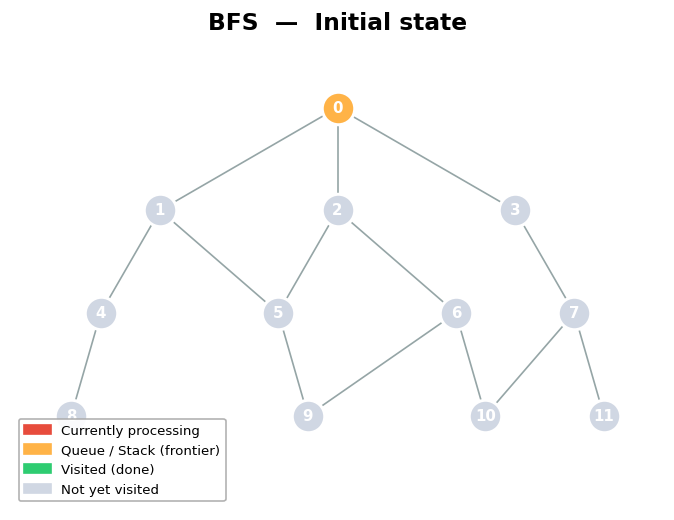
\includegraphics[width=\textwidth]{bfs_step00.png}
    \caption{Initial state (node 0 in queue)}
  \end{subfigure}
  \hfill
  \begin{subfigure}[t]{0.48\textwidth}
    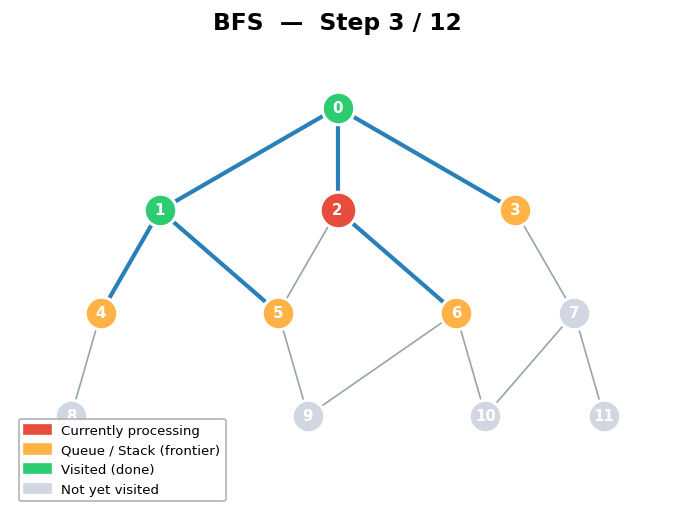
\includegraphics[width=\textwidth]{bfs_step03.png}
    \caption{After visiting node 0: level 1 in queue}
  \end{subfigure}

  \vspace{0.5em}

  \begin{subfigure}[t]{0.48\textwidth}
    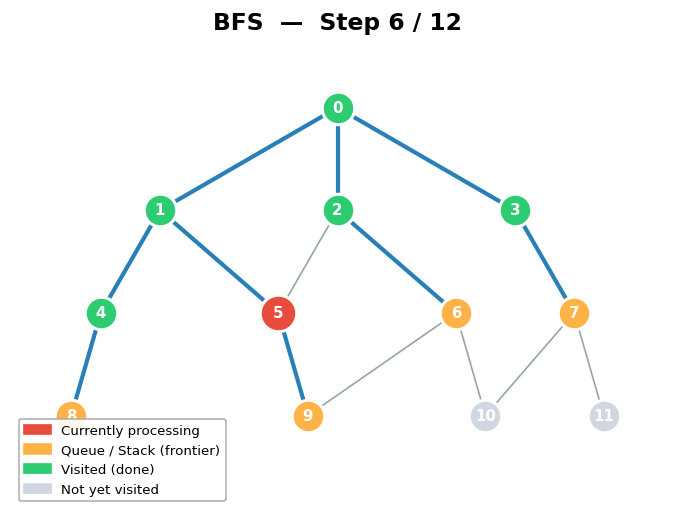
\includegraphics[width=\textwidth]{bfs_step06.png}
    \caption{Mid-traversal: level 2 being processed}
  \end{subfigure}
  \hfill
  \begin{subfigure}[t]{0.48\textwidth}
    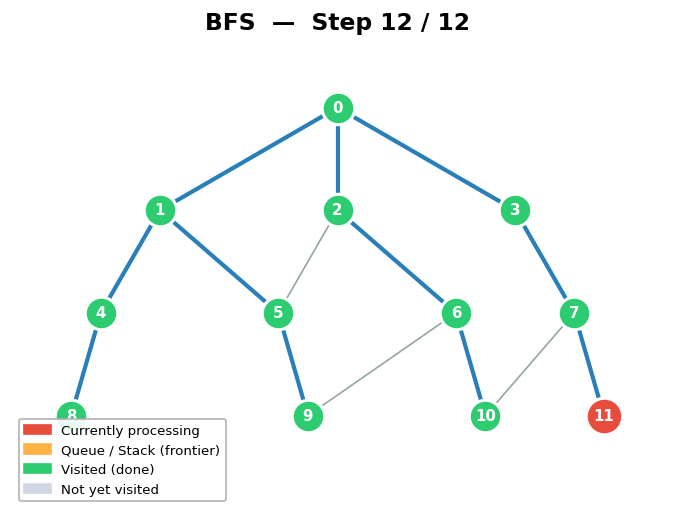
\includegraphics[width=\textwidth]{bfs_step12.png}
    \caption{Final state: all nodes visited}
  \end{subfigure}
  \caption{BFS traversal on the 12-node demo graph (level-by-level expansion).}
  \label{fig:bfs-steps}
\end{figure}

\begin{figure}[H]
  \centering
  \begin{subfigure}[t]{0.48\textwidth}
    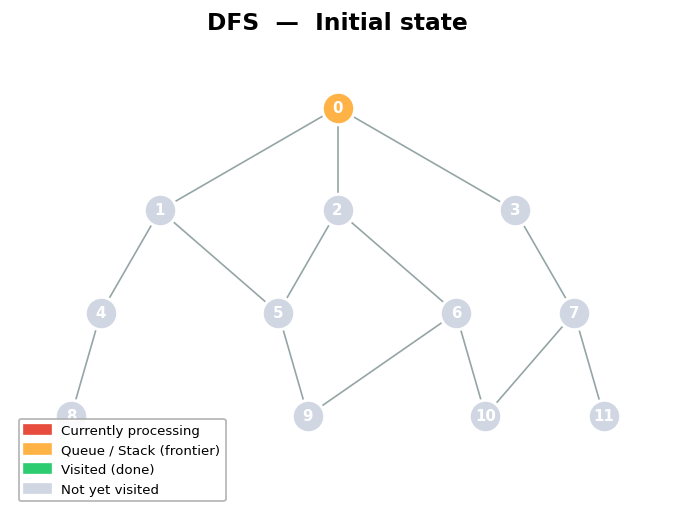
\includegraphics[width=\textwidth]{dfs_step00.png}
    \caption{Initial state (node 0 in stack)}
  \end{subfigure}
  \hfill
  \begin{subfigure}[t]{0.48\textwidth}
    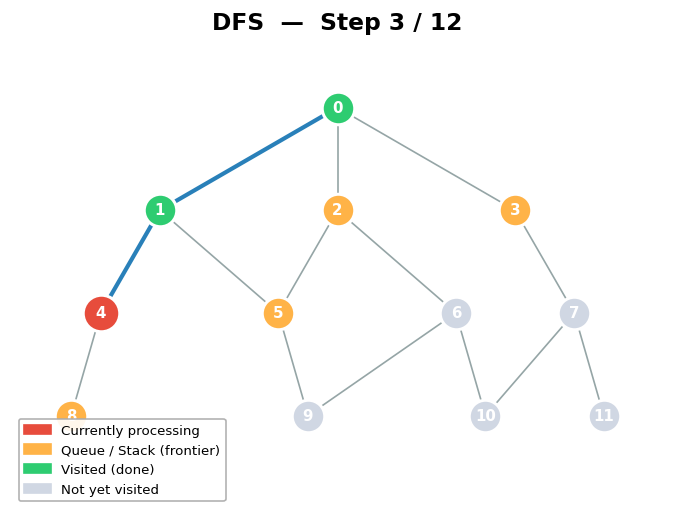
\includegraphics[width=\textwidth]{dfs_step03.png}
    \caption{After visiting 0 $\to$ 1 $\to$ 4: deep path}
  \end{subfigure}

  \vspace{0.5em}

  \begin{subfigure}[t]{0.48\textwidth}
    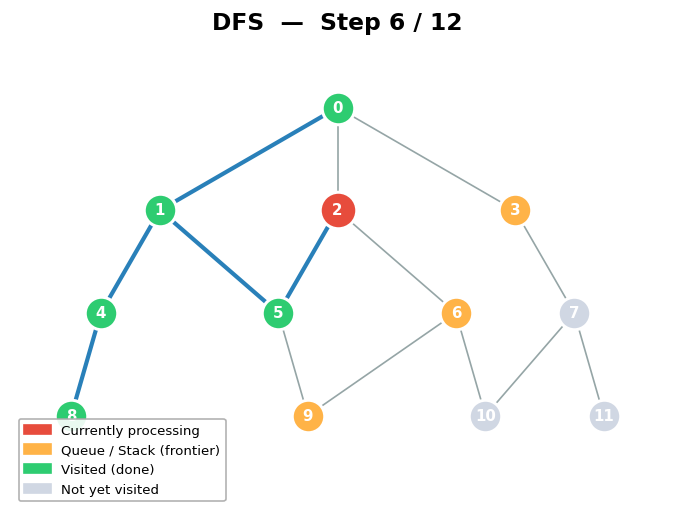
\includegraphics[width=\textwidth]{dfs_step06.png}
    \caption{Backtracking after reaching node 8}
  \end{subfigure}
  \hfill
  \begin{subfigure}[t]{0.48\textwidth}
    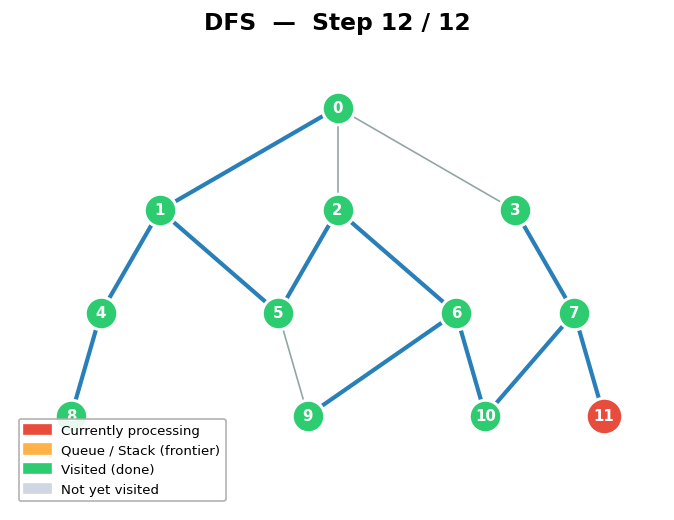
\includegraphics[width=\textwidth]{dfs_step12.png}
    \caption{Final state: all nodes visited}
  \end{subfigure}
  \caption{DFS traversal on the 12-node demo graph (depth-first, backtracking).}
  \label{fig:dfs-steps}
\end{figure}

\noindent The animations make the core difference immediately visible: BFS discovers
all 3 direct neighbours of node 0 before going deeper, while DFS immediately dives
from 0 to 1 to 4 to 8 before backtracking.  Both visit all 12 nodes; only the
\emph{order} and \emph{frontier shape} differ.

% ─── 6. RESULTS AND ANALYSIS ──────────────────────────────────────────────────
\section*{RESULTS AND ANALYSIS}
\addcontentsline{toc}{section}{RESULTS AND ANALYSIS}

\subsection*{Sparse Graphs}
\addcontentsline{toc}{subsection}{Sparse Graphs}

\begin{figure}[H]
  \centering
  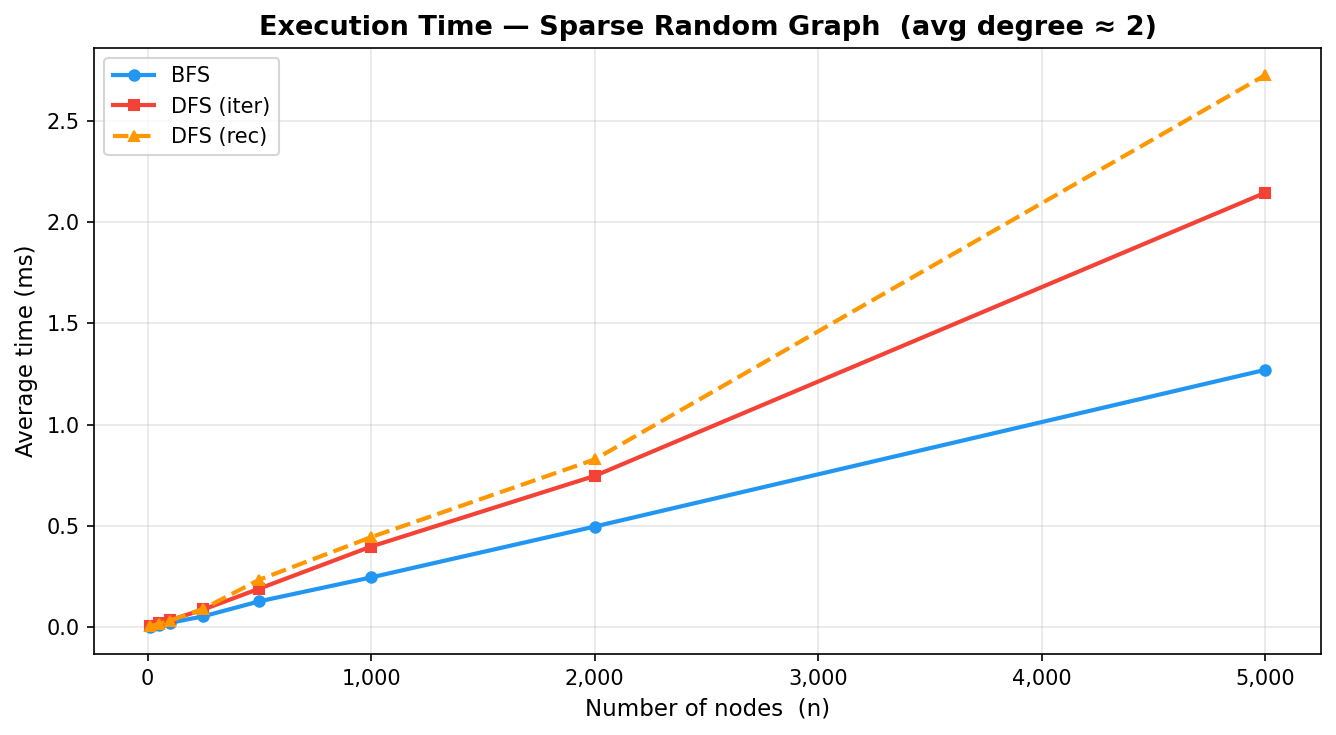
\includegraphics[width=\textwidth]{time_sparse.png}
  \caption{Execution time on sparse random graphs ($n$ up to 5\,000).}
  \label{fig:time-sparse}
\end{figure}

\begin{figure}[H]
  \centering
  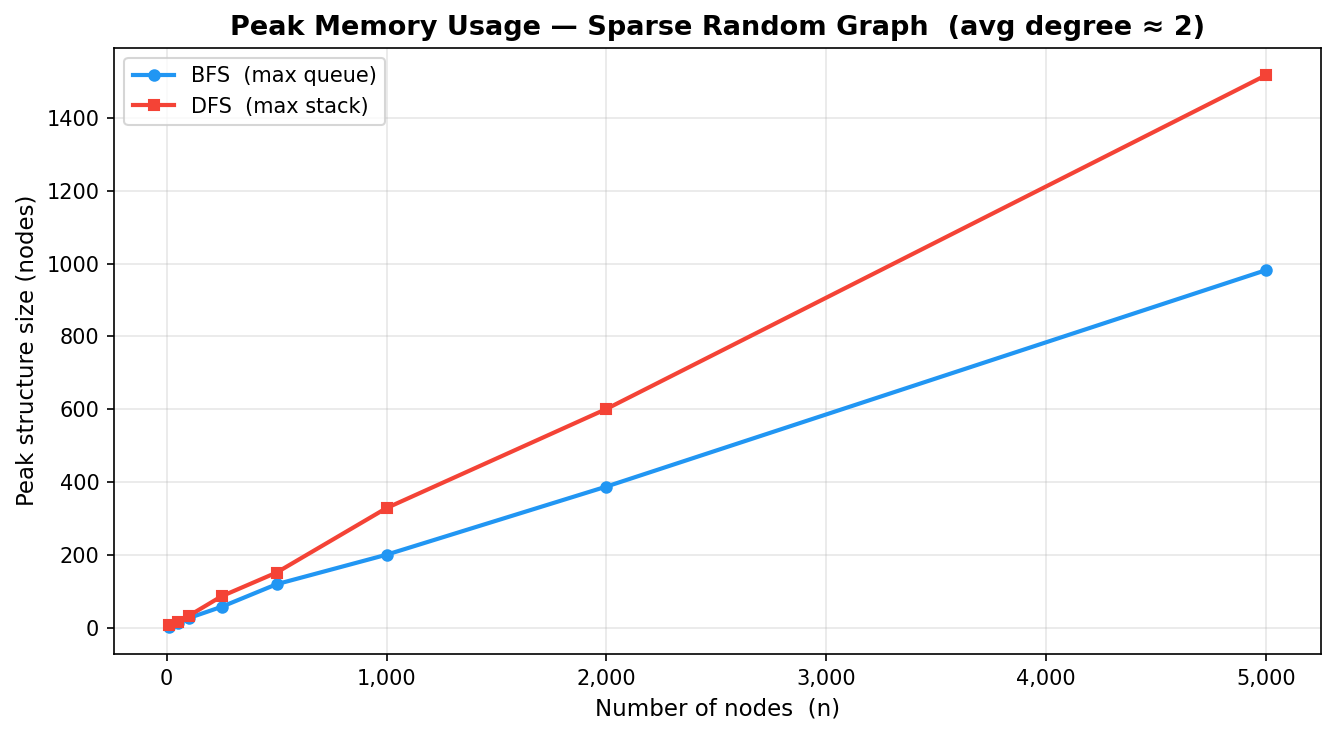
\includegraphics[width=\textwidth]{memory_sparse.png}
  \caption{Peak memory usage on sparse random graphs ($n$ up to 5\,000).}
  \label{fig:mem-sparse}
\end{figure}

On sparse graphs (Figures~\ref{fig:time-sparse}--\ref{fig:mem-sparse}), all three
variants grow linearly with $n$ as expected.  At $n = 5000$, BFS takes
\textbf{1.53\,ms}, DFS-iterative \textbf{2.45\,ms}, and DFS-recursive
\textbf{$\approx$2.45\,ms}.  BFS is roughly \textbf{1.6$\times$ faster} than DFS,
which is attributed to the lower overhead of a deque over a list used as a stack,
and fewer visited-set lookups.  Memory usage is comparable: the BFS queue peaks at
\textbf{982 nodes} and the DFS stack at \textbf{1\,517 nodes} at $n = 5000$.

\subsection*{Dense Graphs}
\addcontentsline{toc}{subsection}{Dense Graphs}

\begin{figure}[H]
  \centering
  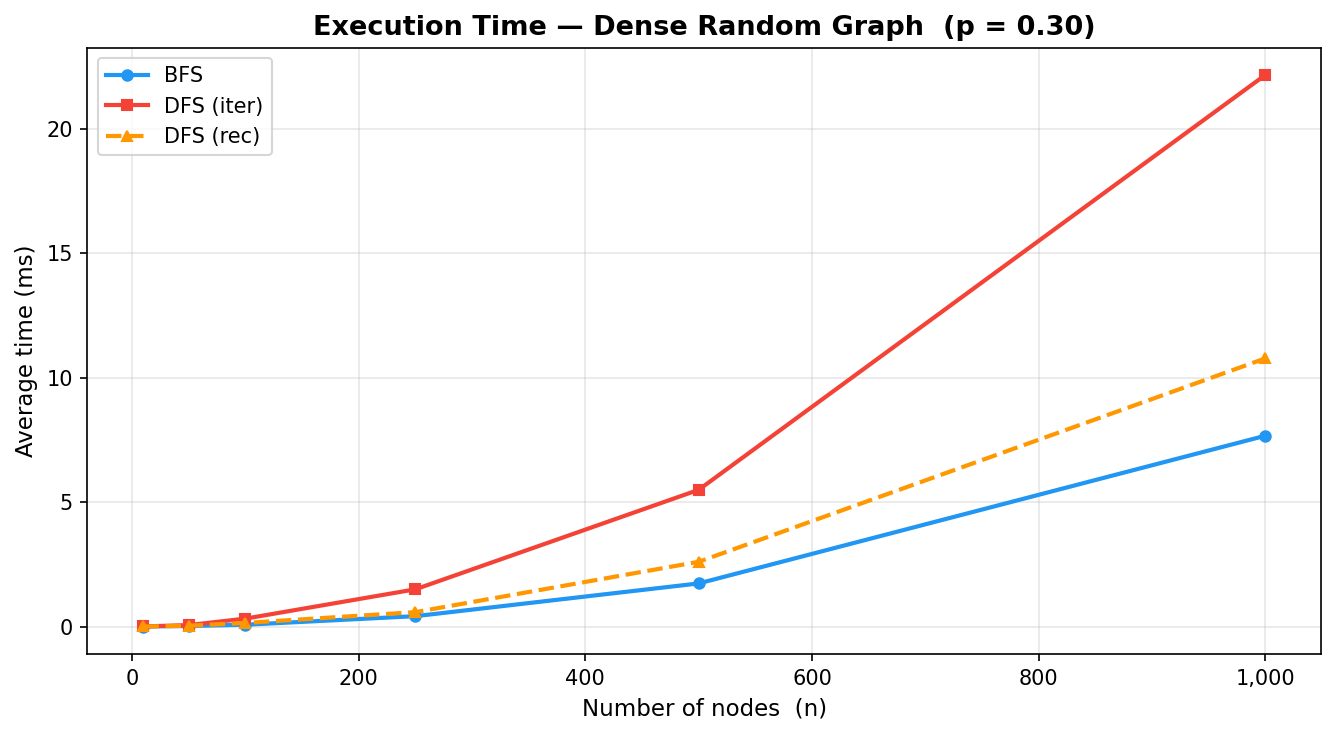
\includegraphics[width=\textwidth]{time_dense.png}
  \caption{Execution time on dense random graphs ($n$ up to 1\,000, $p = 0.30$).}
  \label{fig:time-dense}
\end{figure}

\begin{figure}[H]
  \centering
  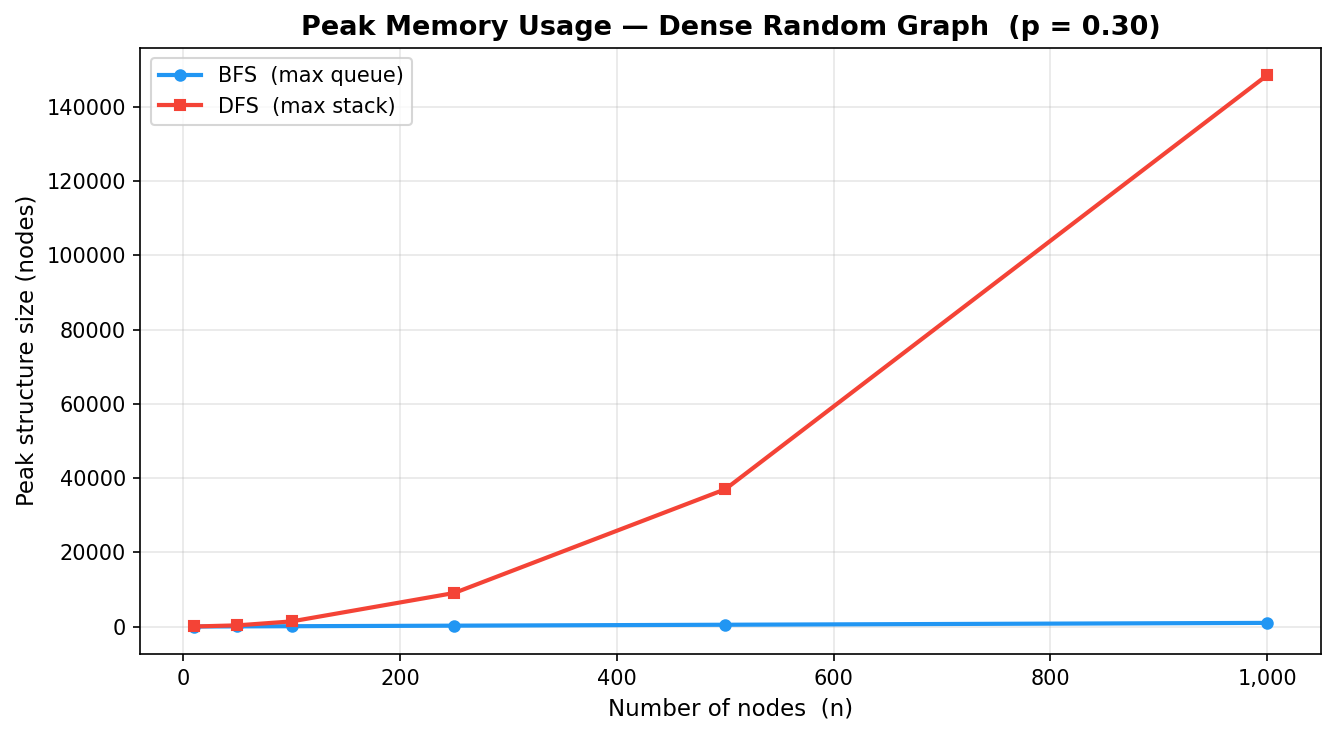
\includegraphics[width=\textwidth]{memory_dense.png}
  \caption{Peak memory usage on dense random graphs ($n$ up to 1\,000).}
  \label{fig:mem-dense}
\end{figure}

Dense graphs (Figures~\ref{fig:time-dense}--\ref{fig:mem-dense}) reveal a dramatic
divergence in memory usage.  At $n = 1000$, the BFS queue peaks at \textbf{984
nodes} (bounded by $V$), while the DFS stack reaches \textbf{148\,562 entries} ---
nearly $\mathbf{150\times}$ more.  The reason is structural: iterative DFS marks
nodes as visited only when they are \emph{popped}, so all unvisited neighbours of
every processed node are pushed onto the stack even if the same node was already
pushed by a previous step.  On a dense graph with $p = 0.30$, each node has on
average $0.30 \times (n-1) \approx 300$ neighbours, causing the stack to accumulate
$O(E)$ entries.

Execution time reflects the same pattern: DFS-iterative is \textbf{5$\times$ slower}
than BFS at $n = 1000$ (\textbf{30.5\,ms} vs \textbf{6.3\,ms}) due to the extra
stack operations and the quadratic edge count.  Both still scale as $O(V + E)$, but
$E = O(n^2)$ for dense graphs, producing the visible super-linear curves.

\subsection*{Binary Trees}
\addcontentsline{toc}{subsection}{Binary Trees}

\begin{figure}[H]
  \centering
  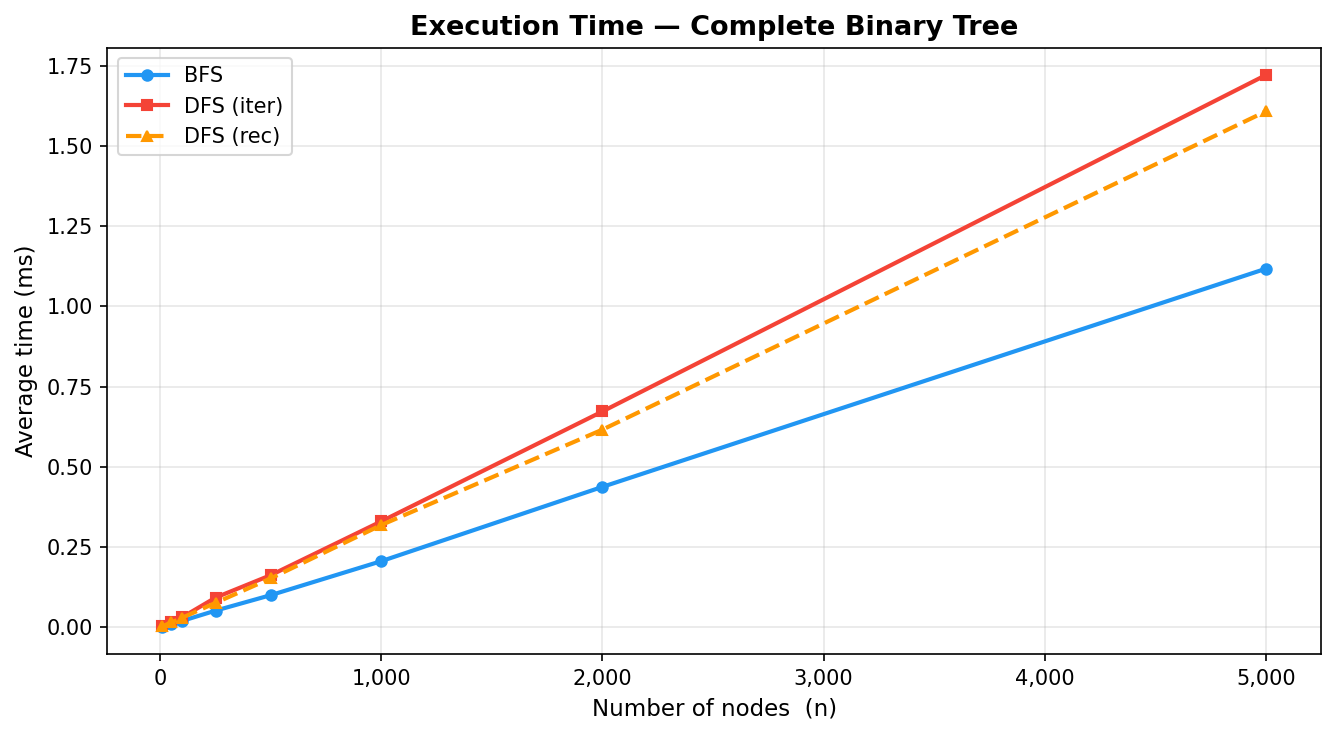
\includegraphics[width=\textwidth]{time_tree.png}
  \caption{Execution time on complete binary trees ($n$ up to 5\,000).}
  \label{fig:time-tree}
\end{figure}

\begin{figure}[H]
  \centering
  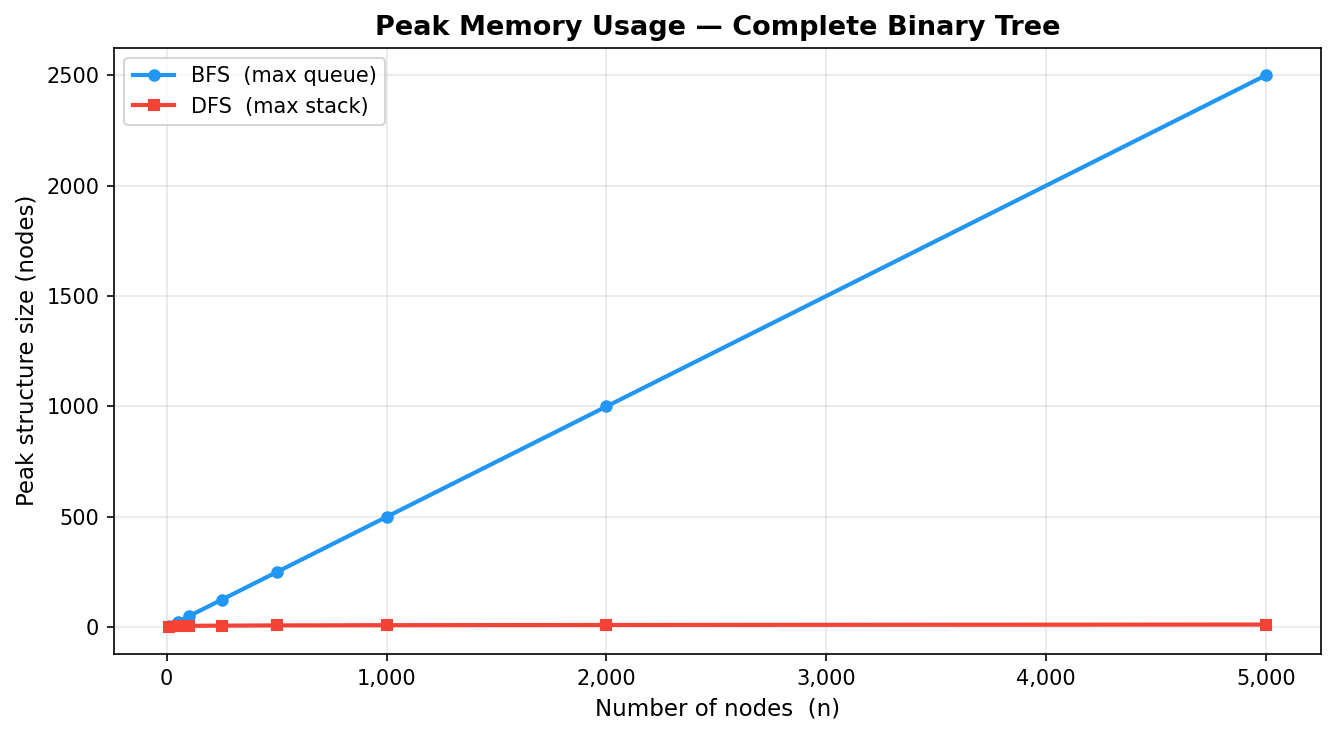
\includegraphics[width=\textwidth]{memory_tree.png}
  \caption{Peak memory usage on complete binary trees ($n$ up to 5\,000). Note the
           dramatic contrast: BFS holds the entire leaf level; DFS only holds the
           path from root to current node.}
  \label{fig:mem-tree}
\end{figure}

The binary tree results (Figures~\ref{fig:time-tree}--\ref{fig:mem-tree}) provide
the most striking memory contrast.  For a complete binary tree of $n$ nodes the
bottom level contains $\approx n/2$ nodes, all of which are in the BFS queue
simultaneously when processing the penultimate level.  This is confirmed empirically:
at $n = 5000$, \textbf{BFS max queue = 2\,500} ($\approx n/2$).

DFS, on the other hand, only keeps the path from the root to the current node on its
stack, which has length $\lfloor \log_2 n \rfloor$.  At $n = 5000$,
\textbf{DFS max stack = 13} ($\log_2 5000 \approx 12.3$).  The ratio is
\textbf{$\approx 192$}, making DFS the memory-efficient choice for tree traversal.

\subsection*{Chain Graphs}
\addcontentsline{toc}{subsection}{Chain Graphs}

\begin{figure}[H]
  \centering
  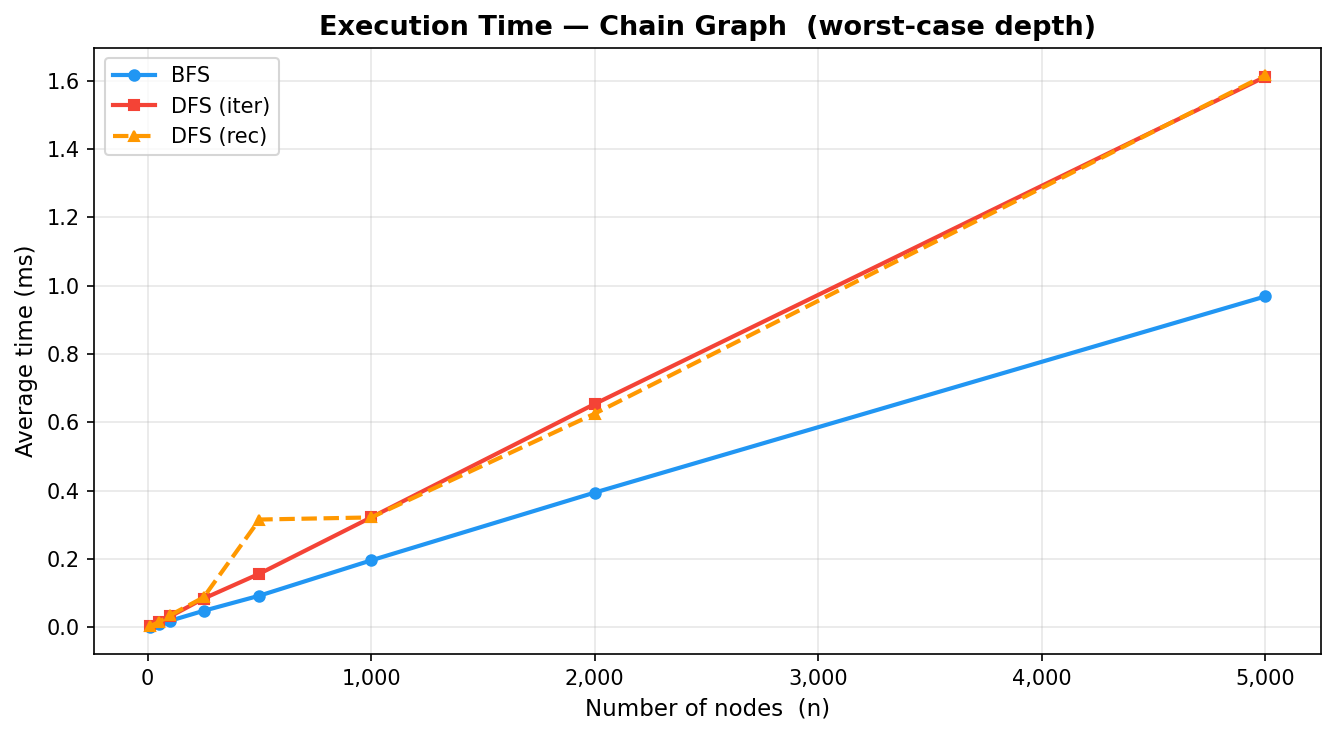
\includegraphics[width=\textwidth]{time_chain.png}
  \caption{Execution time on chain graphs ($n$ up to 5\,000).}
  \label{fig:time-chain}
\end{figure}

\begin{figure}[H]
  \centering
  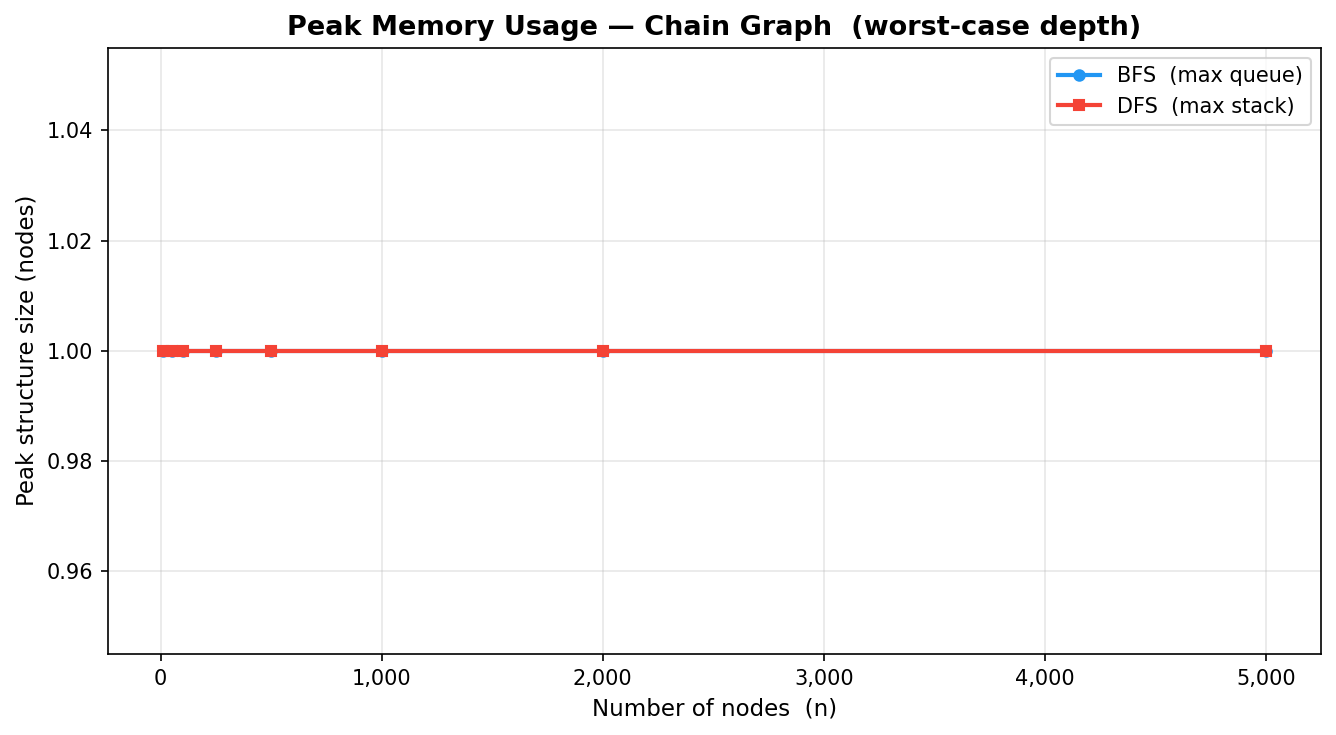
\includegraphics[width=\textwidth]{memory_chain.png}
  \caption{Peak memory usage on chain graphs. Both algorithms maintain a structure of
           size 1 because each node has at most one unvisited neighbour at any step.}
  \label{fig:mem-chain}
\end{figure}

The chain graph (linear path) is notable for its uniform memory behaviour
(Figures~\ref{fig:time-chain}--\ref{fig:mem-chain}).  Both BFS and iterative DFS
maintain a maximum structure size of \textbf{1 node} regardless of $n$: the BFS
queue always contains exactly the next unvisited node, and DFS pops and immediately
pushes only the next node in the chain.

While the explicit-stack depth is O(1), the \emph{recursive} DFS call stack would
grow to $O(n)$ for a chain (one frame per node), which is why the recursive variant
is excluded from large chain benchmarks.  The chain graph thus represents the
worst-case scenario for recursive DFS in terms of call-stack depth and the risk of a
stack-overflow error in languages without tail-call optimisation.

\subsection*{Grid Graphs}
\addcontentsline{toc}{subsection}{Grid Graphs}

\begin{figure}[H]
  \centering
  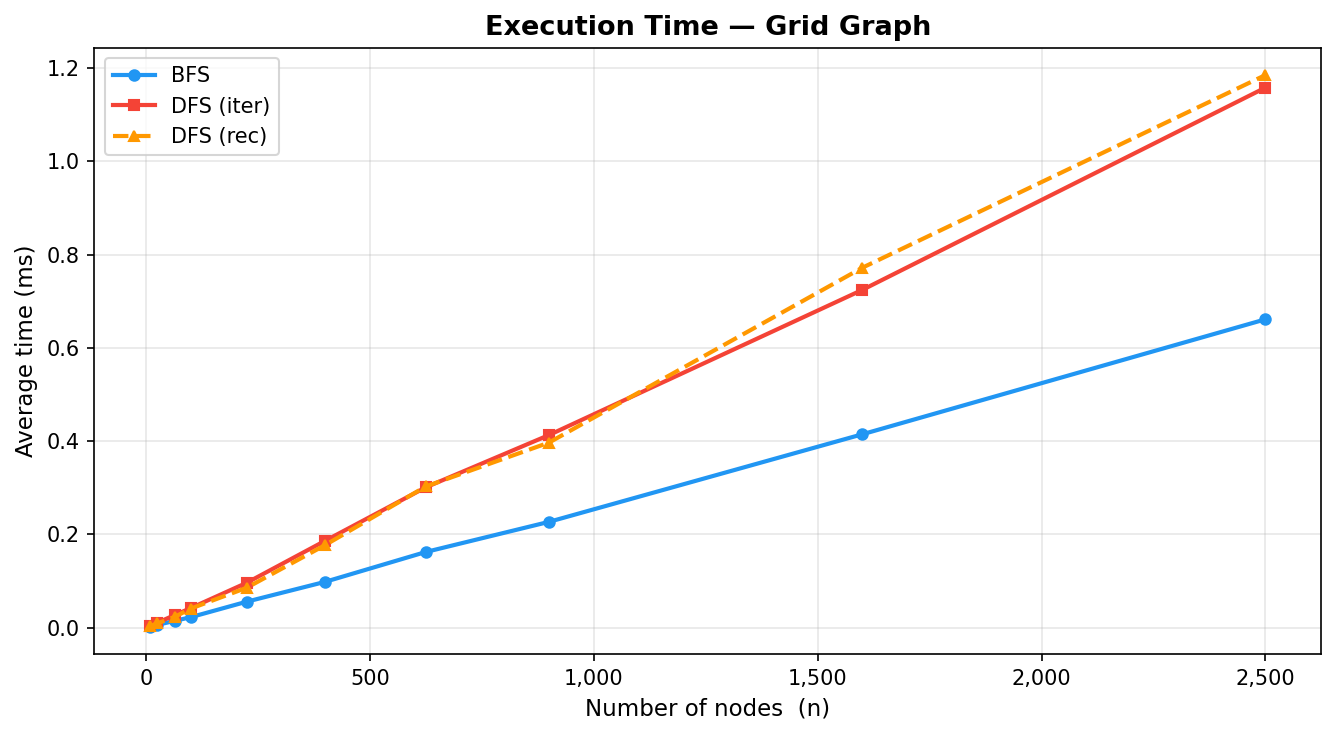
\includegraphics[width=\textwidth]{time_grid.png}
  \caption{Execution time on $\sqrt{n} \times \sqrt{n}$ grid graphs ($n$ up to 2\,500).}
  \label{fig:time-grid}
\end{figure}

\begin{figure}[H]
  \centering
  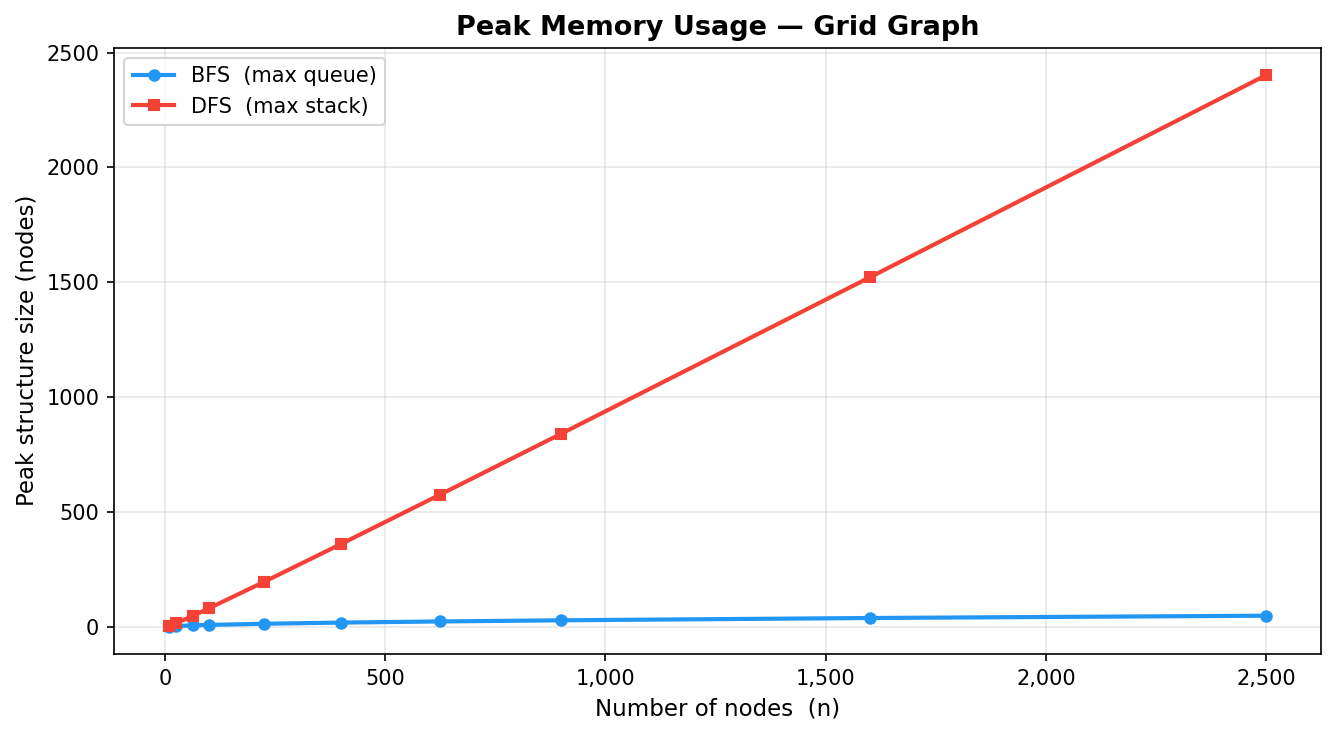
\includegraphics[width=\textwidth]{memory_grid.png}
  \caption{Peak memory usage on grid graphs. BFS queue grows as $O(\sqrt{n})$;
           DFS stack grows as $O(n)$.}
  \label{fig:mem-grid}
\end{figure}

Grid graphs (Figures~\ref{fig:time-grid}--\ref{fig:mem-grid}) expose another
structural characteristic.  BFS expands in concentric ``rings'' from the source
corner, so the frontier at any time spans one ring whose length is proportional to
the grid side $\sqrt{n}$.  At $n = 2500$ (a $50 \times 50$ grid), the peak BFS
queue is \textbf{50} $= \sqrt{2500}$ nodes.

DFS on a grid, however, follows a winding path through the grid and accumulates
unvisited branch points on the stack.  At $n = 2500$, the DFS stack peaks at
\textbf{2\,402 nodes} ($\approx 0.96\,n$) --- nearly the entire grid is held in
the stack simultaneously at some point.

\subsection*{All Graph Types Compared}
\addcontentsline{toc}{subsection}{All Graph Types Compared}

\begin{figure}[H]
  \centering
  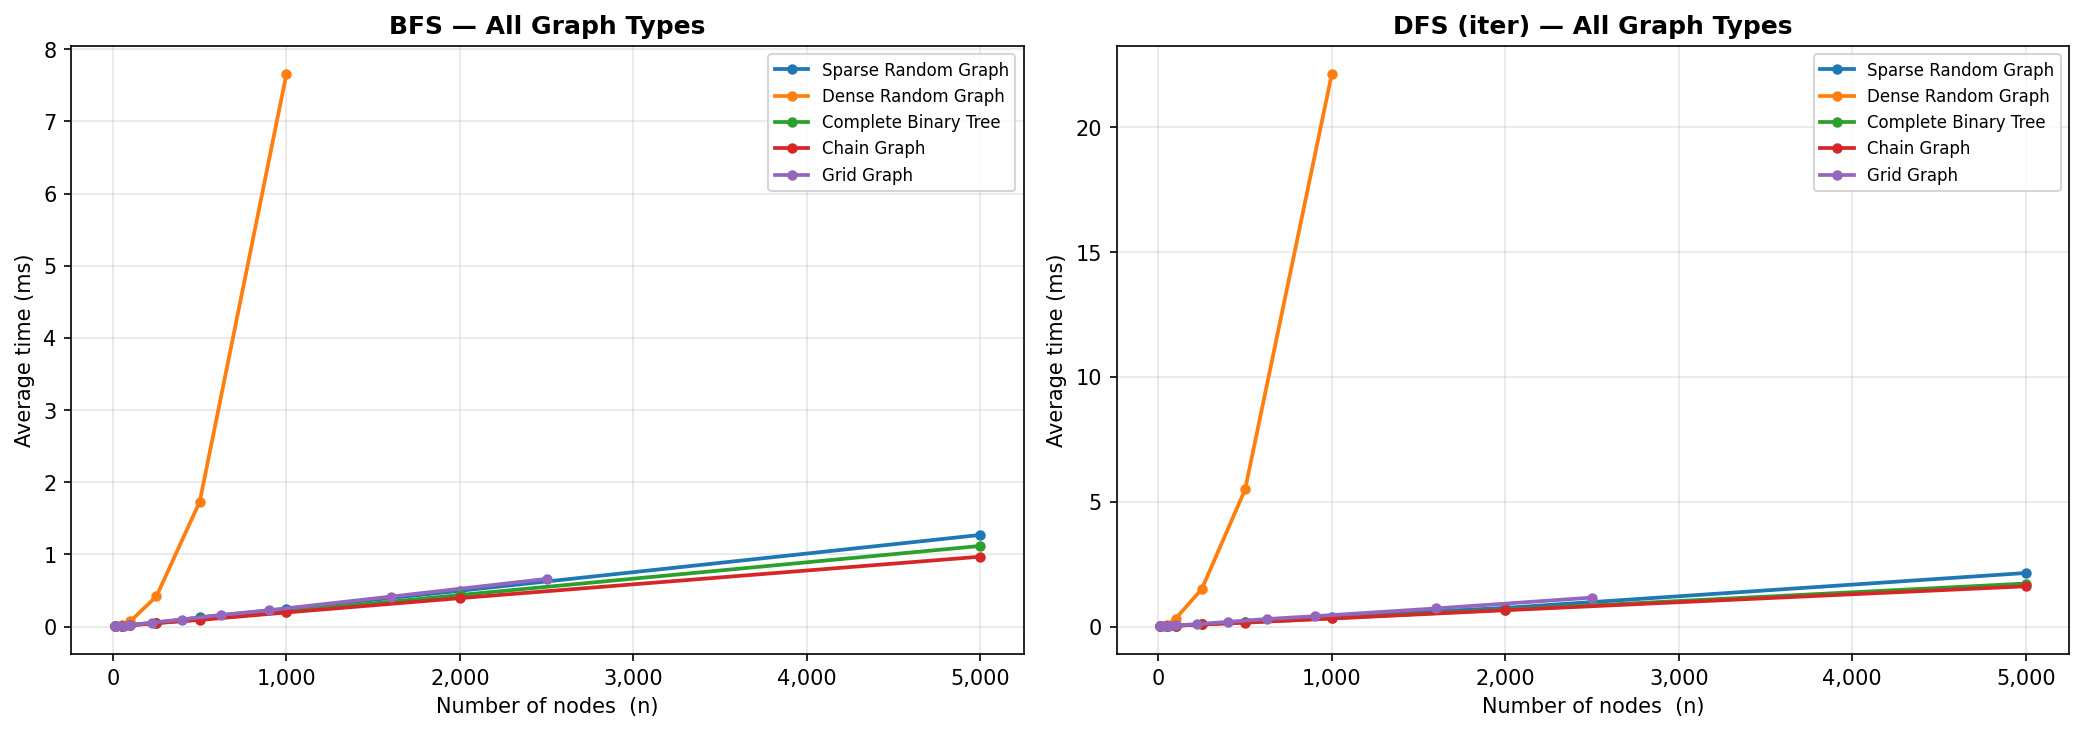
\includegraphics[width=\textwidth]{all_types_comparison.png}
  \caption{BFS (left) and DFS-iterative (right) execution time across all five
           graph types.}
  \label{fig:all-types}
\end{figure}

\begin{figure}[H]
  \centering
  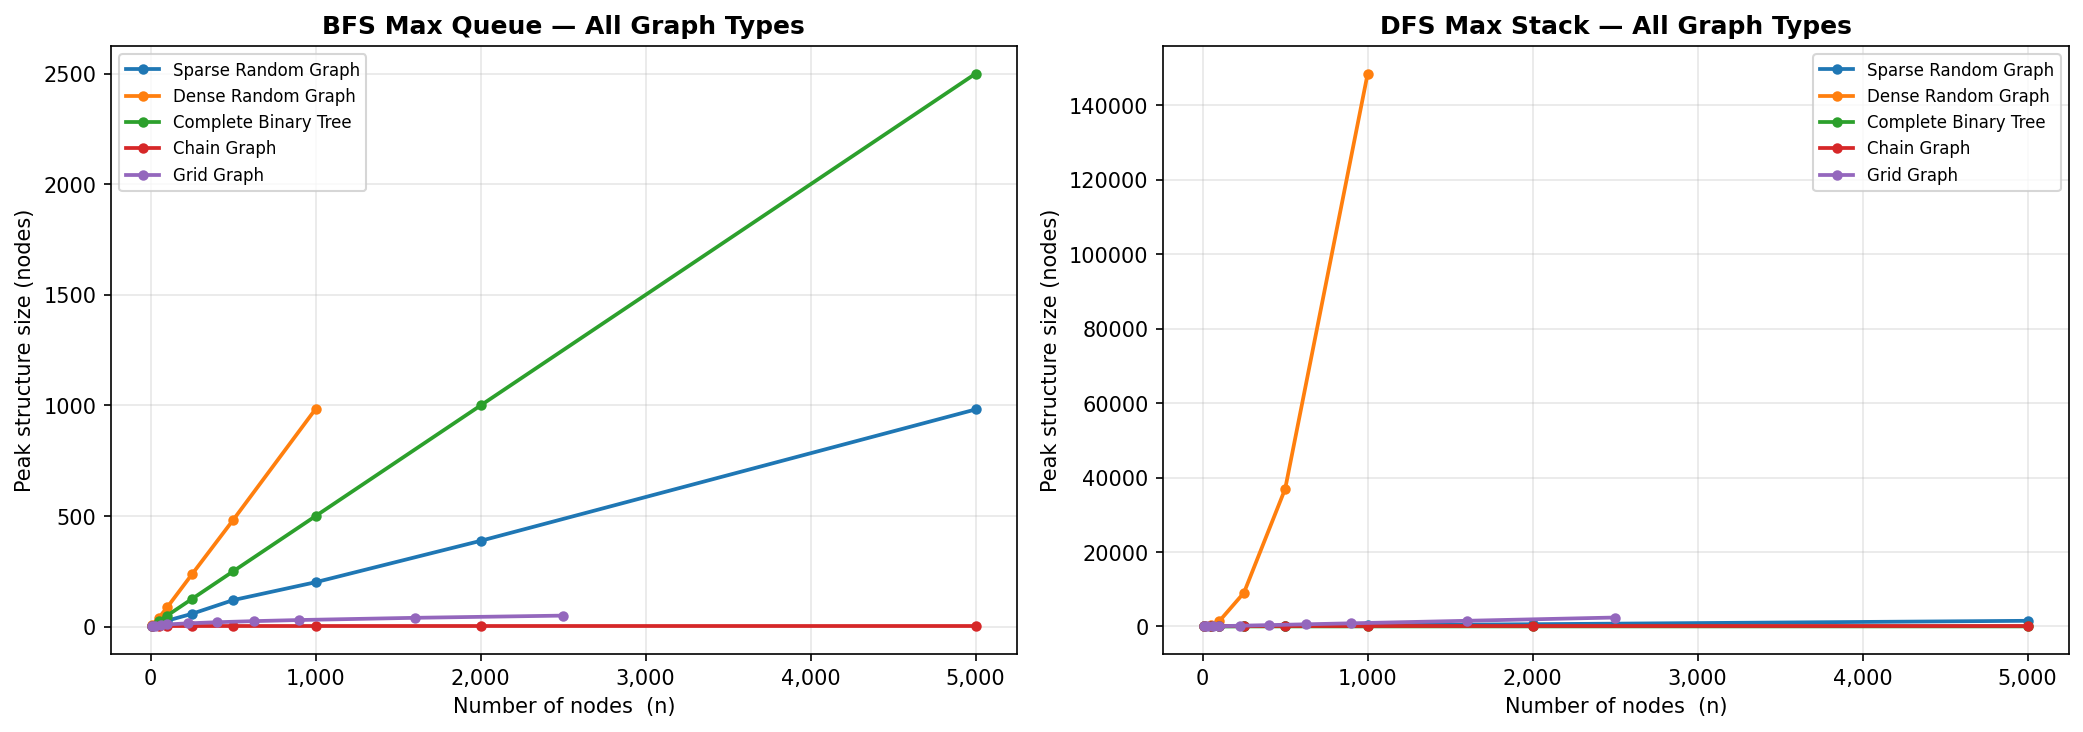
\includegraphics[width=\textwidth]{memory_all_types.png}
  \caption{BFS max-queue (left) and DFS max-stack (right) sizes across all five
           graph types.}
  \label{fig:mem-all}
\end{figure}

Figure~\ref{fig:all-types} confirms that timing is dominated by $E$, not $V$: the
dense-graph curves diverge rapidly because $E = O(n^2)$, while sparse, tree, grid,
and chain all follow similar linear-looking slopes.

Figure~\ref{fig:mem-all} captures the key insight of this laboratory: \emph{the
choice between BFS and DFS does not affect time complexity but has a profound effect
on memory}, and the magnitude depends entirely on the graph's shape.

% ─── 7. EDGE-CASE ANALYSIS ────────────────────────────────────────────────────
\section*{EDGE-CASE ANALYSIS}
\addcontentsline{toc}{section}{EDGE-CASE ANALYSIS}

\hspace{0.8cm} Both algorithms were tested on six edge-case inputs:

\begin{center}
\renewcommand{\arraystretch}{1.4}
\begin{tabular}{llll}
\toprule
\textbf{Scenario} & \textbf{Input} & \textbf{Expected} & \textbf{Result} \\
\midrule
Empty graph        & \texttt{\{\}} (no nodes)          & \texttt{[]} (no visits)           & \checkmark \\
Single node        & \texttt{\{0: []\}}                & \texttt{[0]}                      & \checkmark \\
Disconnected graph & Nodes $\{0,1,2,3\}$, no edges     & Only \texttt{[0]} visited         & \checkmark \\
Self-loop          & \texttt{0 → 0}, \texttt{0 → 1}   & \texttt{[0, 1]}, loop ignored     & \checkmark \\
Complete graph     & $K_5$ (all pairs connected)       & All 5 nodes visited               & \checkmark \\
Cycle graph        & Ring $0\!-\!1\!-\!2\!-\!3\!-\!0$ & All 4 nodes visited, no infinite loop & \checkmark \\
\bottomrule
\end{tabular}
\captionof{table}{Edge-case scenarios, expected outputs, and test results.}
\end{center}

Both BFS and DFS handle all six scenarios correctly.

\textbf{Disconnected graph:} both algorithms only visit the connected component
containing the starting node.  Nodes in other components are simply never reached ---
no error is raised.  If full graph coverage is required (visiting all components), the
caller must iterate over all nodes and start a new traversal for each unvisited node.

\textbf{Self-loops:} the visited-set check prevents re-visiting the same node, so a
self-loop (\texttt{graph[0] = [0, 1]}) is silently ignored --- node 0 is already in
\texttt{visited} when the loop edge is processed.

\textbf{Cycle graph:} both algorithms correctly terminate because visited-set
membership prevents any node from being enqueued/pushed twice (BFS) or processed
twice (DFS).

% ─── 8. CONCLUSION ────────────────────────────────────────────────────────────
\section*{CONCLUSION}
\addcontentsline{toc}{section}{CONCLUSION}

\hspace{0.8cm} Through empirical analysis, BFS and DFS were measured across five
graph types and a wide range of sizes.  The study yields the following practical
conclusions:

\textbf{Time complexity:} both algorithms exhibit $O(V + E)$ runtime.  In practice,
BFS runs approximately \textbf{1.5–2$\times$ faster} than iterative DFS across all
tested graph types, primarily due to the lower overhead of the \texttt{deque}-based
queue and fewer duplicated structure operations.

\textbf{Memory: BFS favours deep graphs, DFS favours wide graphs.}
\begin{itemize}
  \item On a \textbf{binary tree} of 5\,000 nodes, BFS requires a queue of 2\,500
        nodes ($n/2$) while DFS only needs a stack of 13 nodes ($\log_2 n$).
        For hierarchical/tree-shaped data, DFS is drastically more memory-efficient.

  \item On a \textbf{chain} of any length, both BFS and iterative DFS maintain a
        structure of size 1, but \emph{recursive} DFS would grow to $O(n)$ call-stack
        depth.

  \item On a \textbf{grid} ($n$ nodes), BFS frontier grows as $O(\sqrt{n})$ while
        the DFS stack reaches $O(n)$.

  \item On \textbf{dense graphs}, the iterative DFS stack can grow to $O(E)$ due to
        duplicate entries pushed before the visited check, making BFS the safer
        choice for dense inputs.
\end{itemize}

\textbf{Algorithm selection guidance:}
\begin{itemize}
  \item Use \textbf{BFS} when shortest-path distances are needed, when the graph is
        expected to be dense, or when a level-order exploration is required.
  \item Use \textbf{DFS (iterative)} when the graph is tree-shaped or when memory
        usage must be minimised for wide, hierarchical structures.
  \item Avoid \textbf{DFS (recursive)} on graphs with potentially long paths (e.g.,
        chains, degenerate trees) to prevent stack-overflow errors in languages
        without tail-call optimisation, including Python.
\end{itemize}

\vspace{0.5cm}
\noindent\textbf{Repository:} \url{https://github.com/igortacu/AA}

\pagebreak
\end{document}
